% !TeX spellcheck = cs_CZ
\begin{mdframed}[style=mdexam]
\begin{example}
  Generujte signál s lineárně rostoucím kmitočtem "\texttt{chirp signál}", maximální kmitočet
  $f_{max} = 20 Hz$, amplituda $A = 1$, vzorkovaný kmitočtem $f_s = 64 Hz$.

    {\centering
    \captionsetup{type=figure}
     \begin{tabular}{c}
         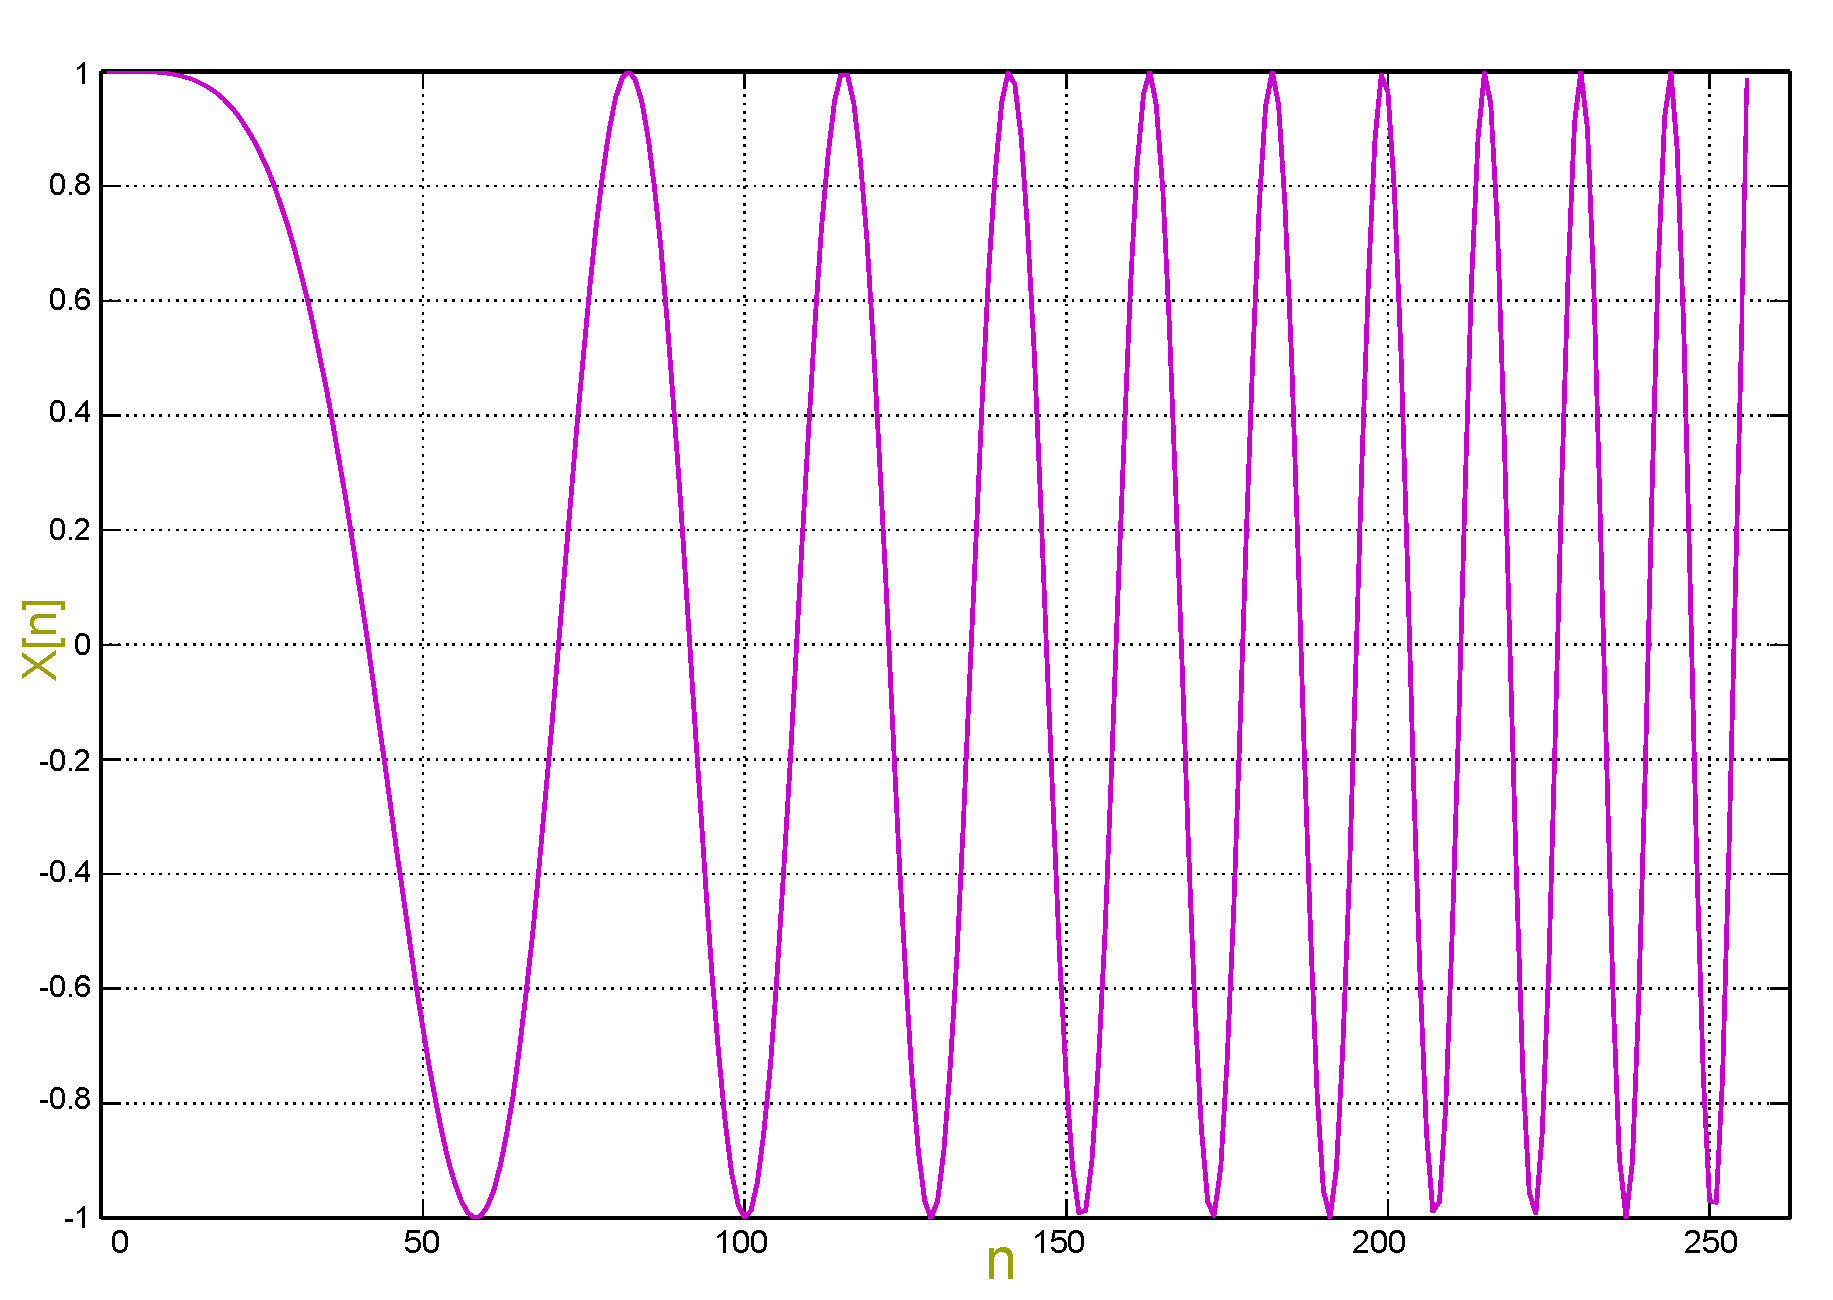
\includegraphics[width=0.8\linewidth]{ces_fig047a.pdf}  \\
         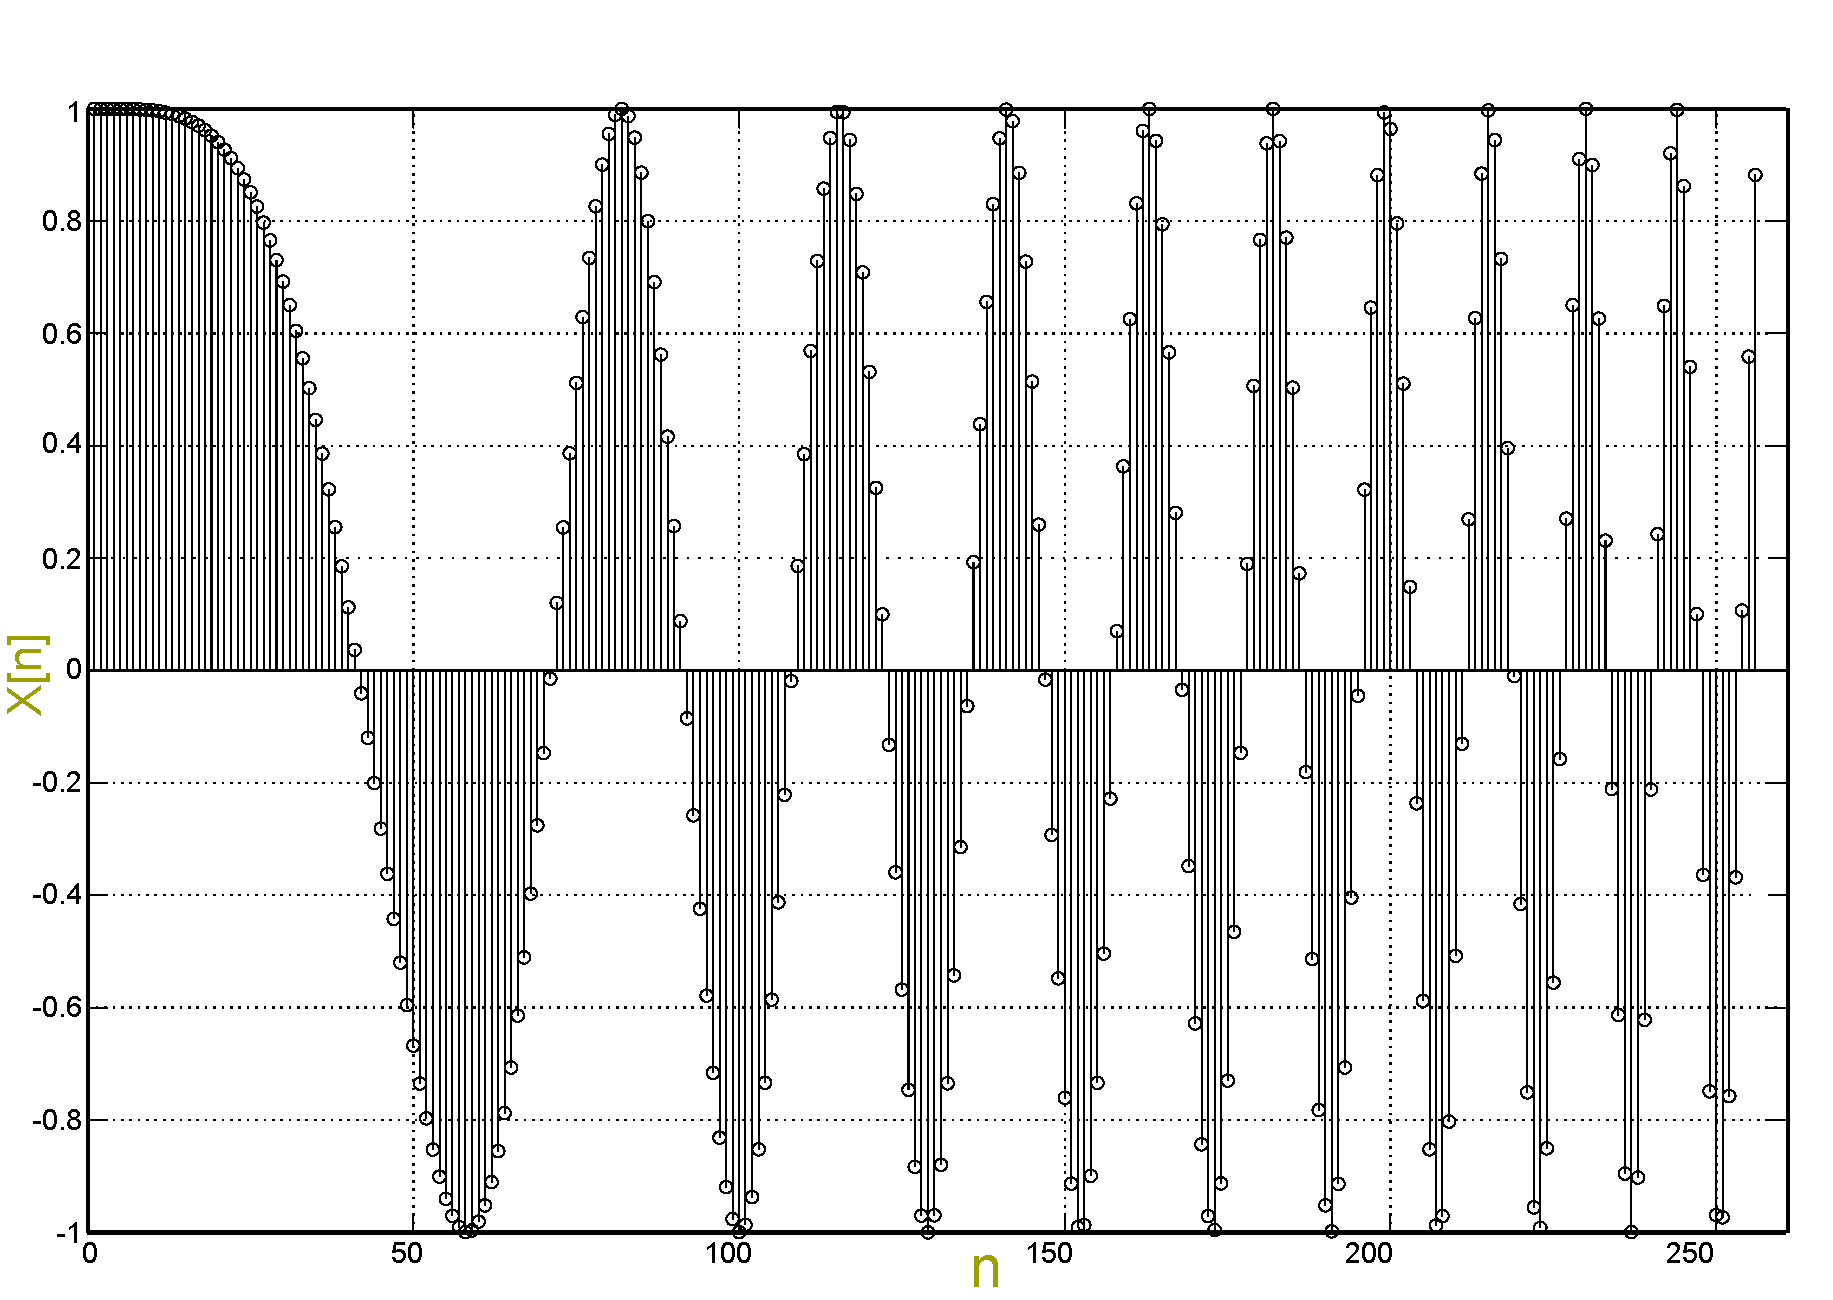
\includegraphics[width=0.8\linewidth]{ces_fig047b.pdf} 
     \end{tabular}  
     \captionof{figure}{Chirp signál: Signál s lineárně rostoucím kmitočtem s maximální
              frekvencí 20 Hz vzorkovaný 254 Hz. Grafická reprezentace číslicových signálů bývá
              buď ve spojité formě (a) nebo v diskrétní formě (b) 
     \label{ces:fig047}}
  \par}
  
  M-file:
  %---------------------------------------------------------------
  \lstinputlisting[%
    style=luaMatlabStyle,
    caption={\texttt{gen\_chirp\_signal.m}. Generuje chirp signál}
    ]{../src/CES/matlab/gen_chirp_signal.m}
  %--------------------------------------------------------------- 
\end{example}
\end{mdframed}